\section{Study 3 - Evaluating Reflection on Design} 

The study explores how interacting with the redesigned telehealth system affects reflection and COPD patients’ activities in self-managing their chronic condition. 

\subsection{Prototype Re-Design}
We made adjustments to the prototype based on findings from Study 2 and developed a web application build on the Bootstrap framework using different Javascript libraries for visualizations (See Worksheets). An introductory dialogue box implemented in the system provided basic information such as (1) it is important to measures under comparable conditions, (2) be aware of context-relevant variables and (3) be aware of sudden changes in symptoms that can be indication of an exacerbation. 

All reflective questions targeted patients’ symptoms and measures, e.g. \textit{Have you previously been able to improve your measures? How?}. Some targeted features of the systems to increase awareness on symptom changes, e.g. \textit{You have several measures that are yellow or red. Is there any improvement since your last measure? (Look at the arrows)}. We chose V1 for long-term reflection based on the idea that it could be of interest for patients interested in seeing relationships between measures and potentially support awareness on deviations \cite{Rivera, Cuttone}. 

\subsection{Methodological and Ethical Considerations}
We had a number of ethical considerations on the design and methodology prior to the study. COPD is a severe condition that comes along with multiple other severe and chronic diseases that patients sometimes live with alone. Research shows that COPD patients are often elderly people with low levels of health literacy \cite{Lisa} and often suffer from anxiety and depression \cite{Who} which has to be taken into account, when designing and studying such patients. From the beginning, we explicitly told all patients that the purpose with the study was to investigate, how patients reflect on symptom changes and not on providing any kinds of support on action. All patients signed a consent form agreeing that they had understood and accepted that their data was not monitored by healthcare professionals. 

We chose to conduct semi-structured interviews as our main method for data collection, focusing on the same methodological considerations as in Study 2. We also included logging and diaries as unobtrusive methods for collecting data about, how patients interact with the system and reflected on their disease during the trial period. We made diary writing optional and ensured that patients prior to the study in the signed consent form accepted that we logged their anonymised data stored on a secured server. 

\subsection{Participants}
Five COPD patients (P1-P5), two male patients (P2, P4) between 67 and 76 years (M: 71.5) and three female patients between 69 and 80 years (M: 75.0), participated in the study. Seven COPD patients initially enrolled, but one male patient dropped out because he did not have surplus energy and because it involved a tablet, while another female patient was hospitalized during the intervention. Patients had lived with a COPD diagnosis in between 7 and 25 years (M: 12) at the time of the study. All patients had either severe or very severe COPD. Two of the female patients (P3, P5) used supplemental oxygen. P3-P5 had multiple other health-related conditions (diabetes, osteoporosis and fibromyalgia). P4 reported color blindness, but ability to distinguish between the colors used in the system, while P5 reported cataract affecting her vision. 

P1 and P5 lived alone, while all the other patients lived with at least a spouse. None of the patients were active on the labour market at the time of the study, but had been holding diverse professions (e.g. teacher, mechanic, cleaning assistant). P2 was the only patient who did not use technology (e.g. computer, tablet or similar) at all. His wife (P2S) was in charge of helping him and also participated in the study. Based on self-assessment, all the other patients used technology either on a daily basis (P1, P4-P5) or 1-6 times weekly (P3) e.g. to check bank accounts, social media, entertainment and similar. P5 had no prior experience with tablets. P1 and P4 had used AF for three months and continued use during our intervention, P2 and P5 previously used THC (for approximately 6 months). P3 had been in a telehealth intervention, where she participated in the control group.  



\begin{figure}[!htb]
 \centering
 \begin{minipage}[b]{0.23\textwidth}
   \includegraphics[width=\textwidth]{img/AL}
   %\caption{Flower one.}
 \end{minipage}
 \hfill
 \begin{minipage}[b]{0.23\textwidth}
   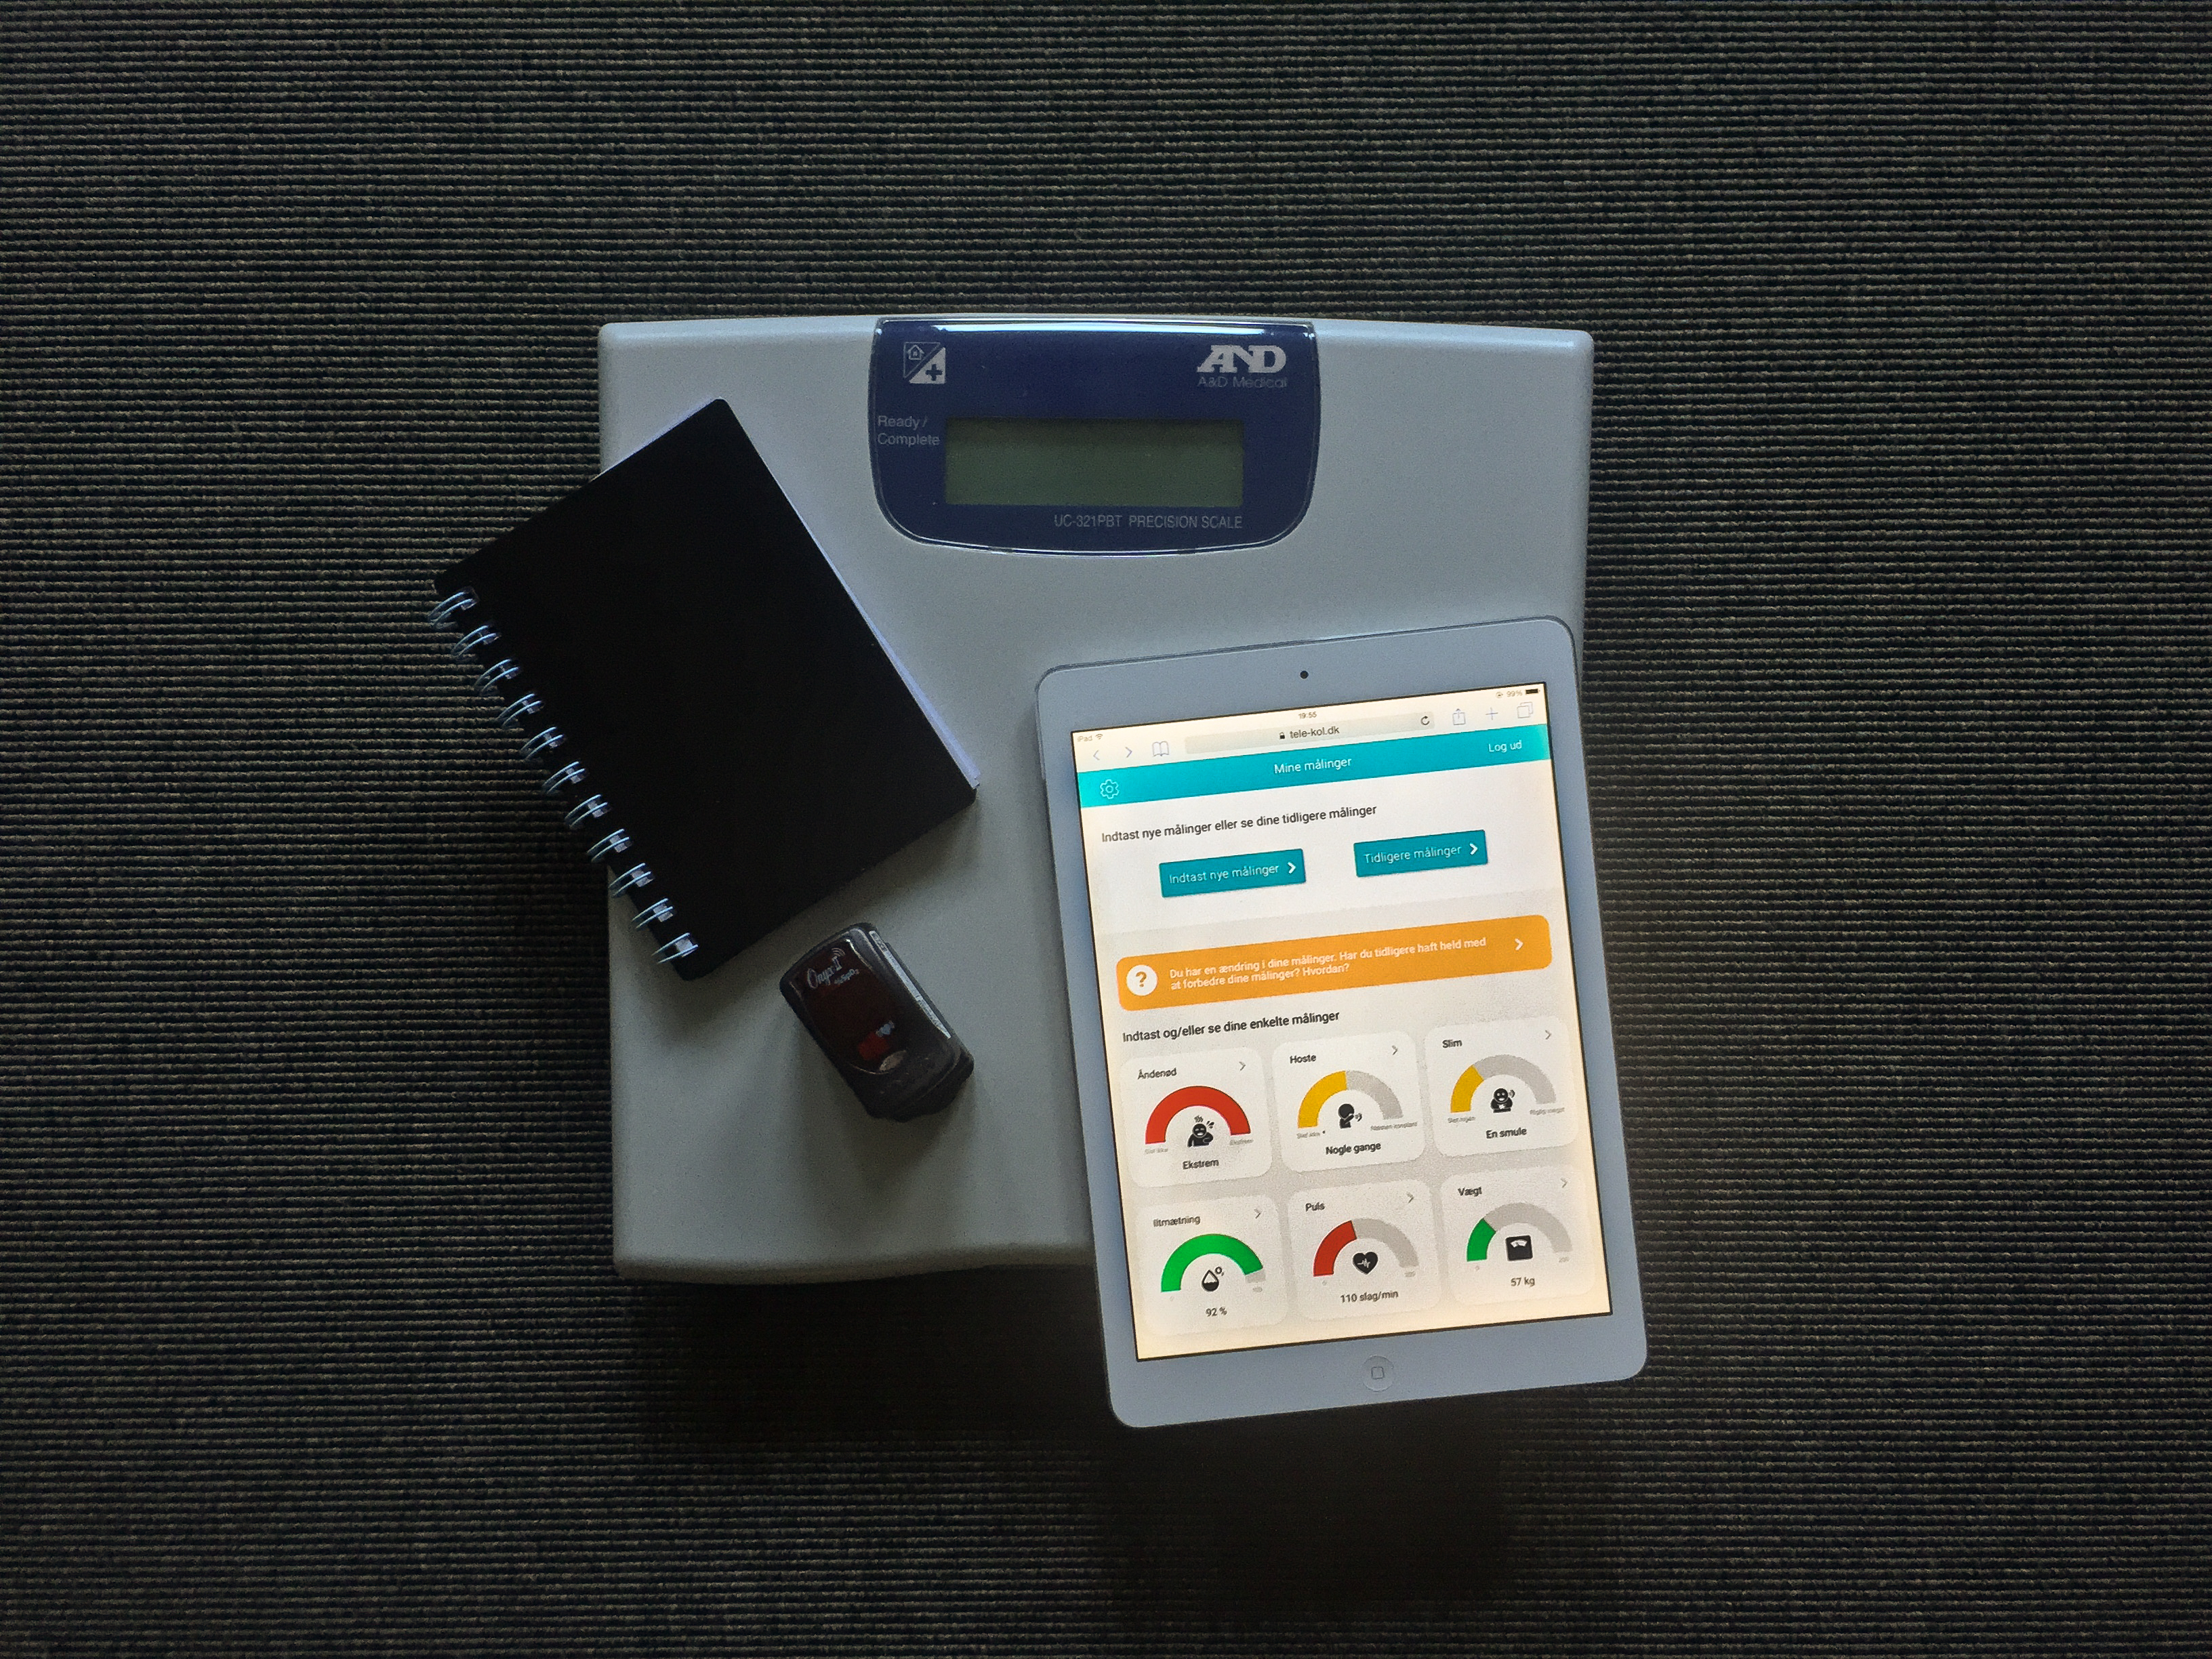
\includegraphics[width=\textwidth]{img/kit}
   %\caption{Flower two.}
 \end{minipage}
  \caption{COPD Patient using TeleKOL (left) and TeleKOL kit (right)}
\end{figure}


\subsection{Procedure}
We recruited participants through contact with Silkeborg Regional Hospital. The only inclusion criteria was that patients had prior telehealth experience. We later found that P3 had only been in the standard care group of a previous telehealth intervention. Our procedure included three steps: 

\textit{Preliminary Data Collection}: After consent over phone, we sent out a letter to all patients with a study information sheet and templates one week before the trial. Patients were asked to fill out template with measures of oxygen saturation, pulse, weight and self-reported dyspnea, cough and phlegm two days that week (preferably with a gap between the days). We input the collected data for each patient in the prototype. 

\textit{Trial Period}: We scheduled initial meetings with patients ensuring that they all had a complete TeleKOL kit (See Figure xx) consisting of a pulse oximeter, weight, diary and iPad with access to the internet and signed a consent form. A facilitator asked patients basic information needed in the system to compute BMI (age and height) and then educated patients in the use of the system (opening the application, submitting data, accessing previous measures and settings). Patients were asked to use the system at least three time a week and encouraged to use it more often along with the diary writing. Patients who also used AF were asked to use the system on days where they did not use AF. We scheduled follow-up meetings with patients 14 days after the trial started. 

\textit{Follow-up interviews}: Two researchers conducted semi-structured interviews with all patients in their home. Each interview lasted between xx and xx minutes. Interviews were audio-recorded after consent from the patients. Patients filled out demographic questionnaires. Meanwhile, one of the researchers read the diaries and prepared interview prompts. Before each interview we prepared screenshots of patients’ dashboard views showing events of interest (e.g. many red color indicators) used to refoster reflection. An interview guide including topics to be discussed, e.g. concrete COPD related activities for managing disease and system use served as the framework. We showed a short video of THC to those patients, who had used it previously, to remind them before we engaged in a discussion on comparing their previous telehealth experience with the system they had used. 

Two researchers transcribed and coded the audio-recordings using an initial code list. We then defined emerging themes through an iterative process of reviewing the codes. 

\subsection{Results}
We present our findings under five themes that provides a structure for presentation. These are (1) system use and barriers for reflection, (2) using measures as health status indicators, (3) feeling empowered in everyday life, (4) questioning and gaining self-knowledge and (5) becoming motivated to self-improve. While some of the themes overlap, there are also noticeable differences related to different levels of reflection. 

\subsubsection{System Use and Barriers for Reflection}
All patients mentioned the agreement with us as the motivation for taking the system into use, except P3 who mentioned doing it, because she wanted to know her current status (\textit{self-knowledge}) and what she could do about it (\textit{self-improvement}). Drawing on patient types found in Study 2, we identified three active patients (P1, P3 and P4) and two passive patients (P2 and P5). Frequency and duration of system use were not indicative of whether patients were active or passive in the trial period. All patients had used the system approximately 4-5 times, except one active patient (P4) who had used it 9 times. Patients used the system between 5.4 and 12.5 minutes per session (M: 9.25). 
 
Passive patients only took the role as data providers when using the system and did not consider it their job to engage in reflective activity of the self-tracked data, e.g. \textit{“we can not do anything except measure”} (P2) and \textit{“if the bright minds can not make sure that I get better, then neither can I do anything about it”} (P5). According to P5, reflecting on self-tracked data involved speculating on things that she did not believe she could change, \textit{“I do not worry about things that I can not change”}, but she already engaged in similar reflective activity using the pulse oximeter to e.g. adjust her supplemental oxygen level, when she did not feel well. 

\subsubsection{Using Measures as Health Status Indicators}
Patients attached importance to their subjective feeling and their engagement in reflective activity on symptom changes depended on whether they felt good or bad. When patients felt good, they did not necessarily see a reason to engage in the reflective activity, because attaching importance to embrace good days were important to them, e.g. \textit{“(if) I actually feel good, then I do not worry about how I felt yesterday”} (P3) and \textit{“that’s not something I walk around and think about .. Life gets too strenuous if you walk around and think about that (a previous bad day)”} (P1). On the other hand not feeling well in the moment triggered reflection, \textit{“if I do not feel like everything is fine, I might start thinking why (...) it depends on how I am feeling”} (P4). 

Patients already used their pulse oximeter to check their current status, clarify whether oxygen saturation was the cause of not feeling well and then initiated action to improve condition (e.g. breathing exercises if oxygen saturation measure is too low). The dashboard provided a similar indication of health status using multiple measures, \textit{“it (dashboard) is a measure of one’s symptoms (...) altogether it of course becomes how you are feeling”} (P1). The self-tracking activity informed and increased the awareness of how patients were feeling, \textit{“I start noticing three times a week, how am I feeling right now?”} (P4). P3 found it helpful to have it visualized what caused her not feeling well, \textit{“you can not even go to the doctor and learn about your status and why (...) that you can here (dashboard)”} (P3). 

\subsubsection{Feeling Empowered in Everyday Life}
Patients felt more empowered in planning and overcoming everyday tasks. P3 mentioned not wanting to make a spectacle out of herself and felt that she could plan to avoid such situations by knowing her current status, \textit{“now I can make up my mind beforehand (whether to go outside in the heat), because I know how it will end, now where I have been told..”} (P3). Similarly, P4 found that it provided with him a feeling of safety knowing that he was within the recommended levels in terms of his measures, which he could see on the dashboard, \textit{“I’m on the right track then. I do not have to worry about going to folk school or something else”} (P3). 

\textit{Social Responsibility:} Active patients who did not live alone (P3, P4) felt socially responsible towards their relatives. \textit{“I can become unsure about how I am feeling.. (...) I do not want to expose my husband and daughter unnecessary (talks about frightening events) it is about balancing..I learn more about that now, so that I do not expose them (relatives)”} (P3). The self-tracking activity made P5 feel self-centred, but he considered it important in order to be able to do what was best for himself and his acquaintances, \textit{“I have to be self-centred (...) I have to do things right for myself and in time, so that I also treat others right”} (P4). 

\subsubsection{Questioning and Gaining Self-Knowledge}
In using the system, some patients had gained insights and self-knowledge that they had not previously been aware of. Patients asked themselves questions, increasing their awareness on causes of symptom changes. Reflective questions in the system triggered reflection in P3. She had identified that weather had an impact on her breathing difficulties, \textit{“(..) with breathlessness, I had not thought there could be other (reasons) .. I just had breathlessness, done. (..) suddenly I realized how much I was affected by the heat (...) it happened when I sat with the system and those questions, asking why?”}. The option to annotate context variables supported seeking causal explanation \textit{“I have started thinking about it (...) I think, ‘no it’s not that (stress)’, talk? No I haven’t talked today .. and then I think ‘it’s the weather’”} (P3).
 
P4 had started reflecting more on the day before and compared it with the presence to assess whether he could improve anything from yesterday, \textit{“I become very conscious about, how did I feel yesterday? Do I also feel like that today?”} (P4).

Using the system had a transformative effect on P3, who had obtained a new perspective on her disease after using the system and an understanding of, what the measures meant. She felt that having COPD in many years had made her passive and lost hope on being able to do something. 

\textit{“My memory has been stuck, so I thought that is just how it is.. You give up a little and get tired of it (...) without doing anything about it, because nobody says anything.. but this (the system) does. It makes you aware about the situation (...) My doctor always told me that it is all because of my condition. The system makes me think that he is not right. I might have to make demands, then I might get better.”} (P3) 

\subsubsection{Becoming Motivated to Self-Improve}
Active patients (2/3) started setting goals to improve measures. This involved seeking new knowledge, \textit{“I’ve tried to acquaint with BMI because I wanted to have a goal to follow.. (because) I wondered about the arrows (in the system)”} (P4). 

P3 had not previously been aware of the severity of her weight problems had become aware of the need of improving her condition, \textit{“I have not thought about it before, but when you suddenly get it in writing (...) being confronted with it, I have to do something about it (...) it’s for my own good”} (P3). She had started making changes to her eating habits in order to lose weight (eating less, thinking about what she eats, etc.) and mentioned being more aware of engaging in proactive behaviour, \textit{“cough, that’s about getting better at using the PEP device.. Not just saying, ‘oh, you are running into a pneumonia, now you have to use it’, it’s about using it (PEP device) several times a day”}. 

Patients used color indicators and arrows in combination as indicators of status and progress towards goal, “I want all of them to be green and that things are making progress \textit{(...) when the arrows are pointing down I assume it is not so good, that’s the wrong way”} (P4).  Seeing the progress and that it paid off to change her behaviours, motivated P3 to ease off medication intake, which she had tried several times in the past without success. \textit{“They had difficulties easing me off because I have had high doses for so many years (..) but this time I thought (...) now you have to stop (...) I did .. I took some days and then it was over”} (P3). 

\textit{Actionable Advice}: Both P1 and P3 requested actionable advice on what they could do to improve their conditions. P3 needed advice on how to progress towards her goal of losing weight taking into account her other health-related conditions “to get help when you also have diabetes, that would be nice”. P1 mentioned needing actionable advice on improving measures, \textit{“when you sit alone, have breathing difficulties, you cough and you have phlegm, you think, what can I do? It is the alpha and omega”}. 
\subsection{Discussion}


\subsection{Conclusion}

